\documentclass{article}
\usepackage{tikz}
\usepackage{siunitx}
\usepackage{circuitikz}
\begin{document}
% european代表欧洲使用的电路符号. 列表如下:
%   1)european - 欧洲电路符号
%   2)american - 美国电路符号
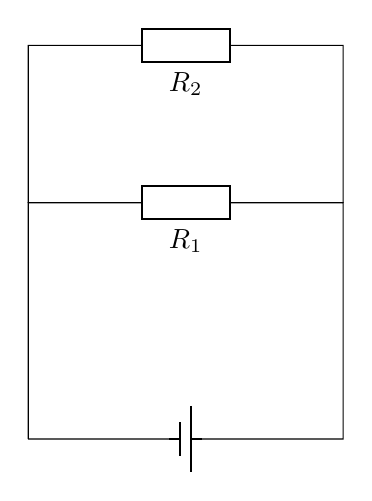
\begin{tikzpicture}[european]
    % 元器件列表:
    %   1.battery1 - 电源,方向不对,需要使用invert反转方向
    %   2.R - 电阻
    %   3.pR - 滑动变阻器
    %   4.D - 二极管
    %   5.leD - 发光二极管
    %   6.rmeter,t=A - 电流表
    %   7.rmeter,t=V - 电压表
    %   8.C - 电容
    %   9.normal open switch - 开关
    %   10.L - 电感器
    % 需要配合元器件使用的符号(可以前置short,代表不显示的元器件)
    %   1.-* - 在线条末尾画一个实心圆点
    %   2.o- - 在线条开始画一个空心圆
    % 元器件操作
    %   1.invert - 组件左右翻转
    %   2.mirror - 组件上下成镜像
    \draw (0,0) to[battery1,invert] (4,0) -- (4,3) to[R=$R_1$] (0,3) -- (0,0);
    \draw (4,3) -- (4,5) to[R=$R_2$] (0,5) -- (0,3);
\end{tikzpicture}\\\vspace{1cm}

% 滑动变阻器
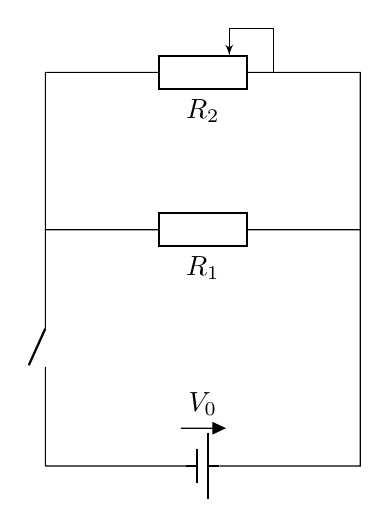
\begin{tikzpicture}[european]
    \draw (0,0) to[battery1,invert,v=$V_0$] (4,0) -- (4,3) to[R=$R_1$] (0,3) to[normal open switch,mirror] (0,0);
    % wiper pos指定滑动变阻器的位置;name为滑动变阻器名称,用于后续引用
    \draw (4,3) -- (4,5) to[pR=$R_2$,mirror,wiper pos=0.2,name=resis] (0,5) -- (0,3);
    % wiper代表滑动变阻器的滑动杆接触点
    \draw (resis.wiper) -| (2.9,5);
\end{tikzpicture}\\\vspace{1cm}

% 元器件的相关内容
%   1.labels - 元器件名称
%   2.annotations - 元器件注解
%   3.voltages - 两端电压
%   4.currents - 电流
%   5.flows - 电路外指示电流
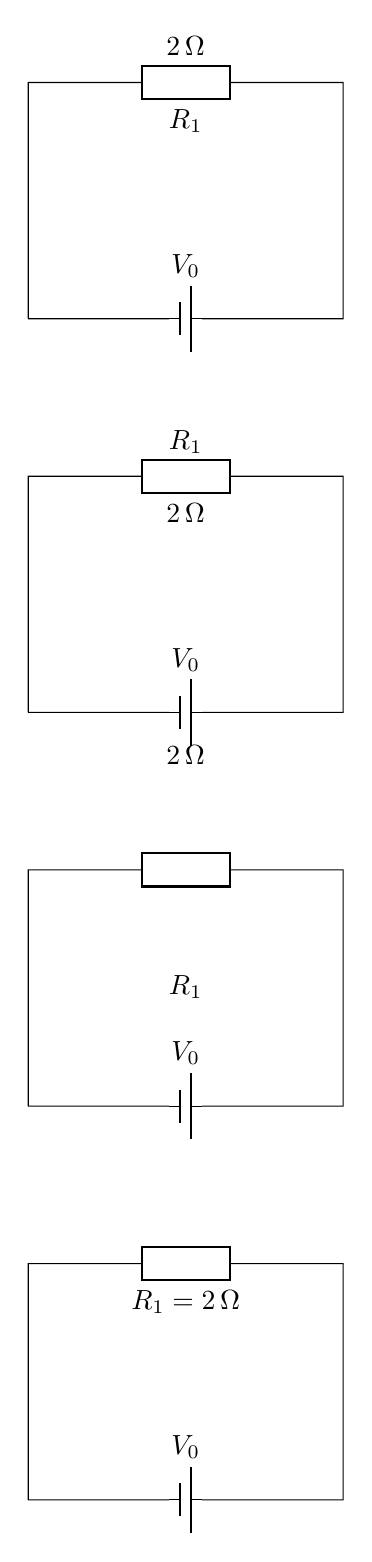
\begin{tikzpicture}[european]
    % label与annotation
    \draw (0,0) to[battery1,invert,l=$V_0$] (4,0) -- (4,3) to[R,l=$R_1$,a=\SI{2}{\ohm}] (0,3) -- (0,0);

    % 在从左到右的电路图中,默认label在元器件上方,annotation在元器件下方
    % 使用以下符号修改label和annotation上下方位置:
    %   1)_ - 将相关内容放置到元器件下方(从左到右)
    %   2)^ - 将相关内容放置到元器件上方(从左到右)
    \draw[yshift=-5cm] (0,0) to[battery1,invert,l=$V_0$] (4,0) -- (4,3) to[R,l_=$R_1$,a^=\SI{2}{\ohm}] (0,3) -- (0,0);

    % 使用以下修改label和annotation距离元器件的距离:
    %   1)label distance - label与元器件的距离
    %   2)annotation distance - annotation与元器件的距离
    \draw[yshift=-10cm] (0,0) to[battery1,invert,l=$V_0$] (4,0) -- (4,3) to[R,l=$R_1$,a=\SI{2}{\ohm},label distance=2cm,annotation distance=1cm] (0,3) -- (0,0);

    % 当label和annotation内包含'='和','时,会出现错误,需要使用{}限定
    \draw[yshift=-15cm] (0,0) to[battery1,invert,l=$V_0$] (4,0) -- (4,3) to[R,l={$R_1=\SI{2}{\ohm}$}] (0,3) -- (0,0);
\end{tikzpicture}\\\vspace{1cm}

% voltage dir=RP可以使用正确电源元器件正负极方向,正确电流方向
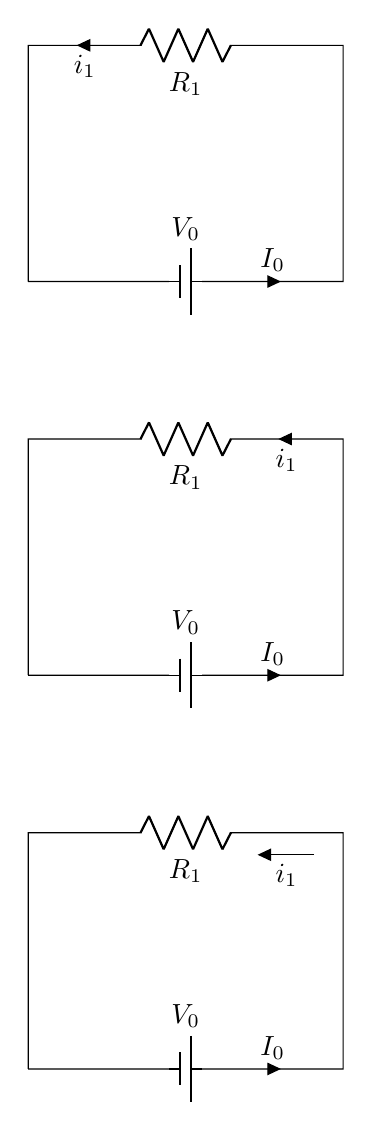
\begin{tikzpicture}[voltage dir=RP]
    % current与flow
    \draw (0,0) to[battery1,l=$V_0$,i=$I_0$] (4,0) -- (4,3) to[R,l=$R_1$,i=$i_1$] (0,3) -- (0,0);

    % 电流标记的方向(标签上下方按照从左到右的方向). 列表如下:
    %   1)^> - 先显示元器件,再显示正向箭头,箭头在标签的上方. 默认
    %   2)^< - 先显示元器件,再显示反向箭头,箭头在标签的上方
    %   3)_> - 先显示元器件,再显示正向箭头,箭头在标签的下方
    %   4)_< - 先显示元器件,再显示反向箭头,箭头在标签的下方
    %   5)>^ - 先显示正向箭头,再显示元器件,箭头在标签的上方
    %   6)>_ - 先显示正向箭头,再显示元器件,箭头在标签的下方
    %   7)<^ - 先显示反向箭头,再显示元器件,箭头在标签的上方
    %   6)<_ - 先显示反向箭头,再显示元器件,箭头在标签的下方
    \draw[yshift=-5cm] (0,0) to[battery1,l=$V_0$,i=$I_0$] (4,0) -- (4,3) to[R,l=$R_1$,i>^=$i_1$] (0,3) -- (0,0);

    % flows标记与电流标记类似
    \draw[yshift=-10cm] (0,0) to[battery1,l=$V_0$,i=$I_0$] (4,0) -- (4,3) to[R,l=$R_1$,f>^=$i_1$] (0,3) -- (0,0);
\end{tikzpicture}\\\vspace{1cm}

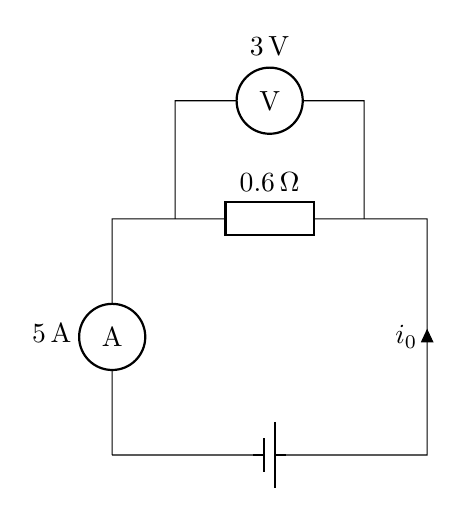
\begin{tikzpicture}[european]
    % 常用单位列表:
    %   \ampere - 电流单位,安倍
    %   \volt - 电压单位,伏特
    %   \ohm - 电阻点位,欧姆
    \draw (0,0) to[battery1,invert] (4,0) to[short,i=$i_0$] (4,3) to[R,a=$\SI{0.6}{\ohm}$] (0,3) to[rmeter,t=A,a=$\SI{5}{\ampere}$] (0,0);
    \draw (3.2,3) -- (3.2,4.5) to[rmeter,t=V,a=$\SI{3}{\volt}$] (0.8,4.5) -- (0.8,3);
\end{tikzpicture}
\end{document}
